% easychair.tex,v 3.4 2015/12/10

\documentclass{easychair}
%\documentclass[EPiC]{easychair}
%\documentclass[debug]{easychair}
%\documentclass[verbose]{easychair}
%\documentclass[notimes]{easychair}
%\documentclass[withtimes]{easychair}
%\documentclass[a4paper]{easychair}
%\documentclass[letterpaper]{easychair}

\usepackage{doc}
\usepackage{comment}
\usepackage{todonotes}
% use this if you have a long article and want to create an index
% \usepackage{makeidx}

% In order to save space or manage large tables or figures in a
% landcape-like text, you can use the rotating and pdflscape
% packages. Uncomment the desired from the below.
%
% \usepackage{rotating}
% \usepackage{pdflscape}

% Some of our commands for this guide.
%
\newcommand{\easychair}{\textsf{easychair}}
\newcommand{\miktex}{MiK{\TeX}}
\newcommand{\texniccenter}{{\TeX}nicCenter}
\newcommand{\makefile}{\texttt{Makefile}}
\newcommand{\latexeditor}{LEd}
\usepackage[ruled]{algorithm}
\usepackage{algpseudocode}
\theoremstyle{theorem}
\newtheorem{theorem}{Theorem}

\theoremstyle{remark}
\newtheorem*{remark}{Remark}
%\makeindex

%% Front Matter
%%
% Regular title as in the article class.
%
\title{Benchmarks for Verification of Autonomous Vehicles }


% Authors are joined by \and. Their affiliations are given by \inst, which indexes
% into the list defined using \institute
%
\author{
Matthew O'Kelly\inst{1}
\and
    Houssam Abbas\inst{1}
\and
  Aditya Pinapala \inst{1}
\and
  Soonho Kong \inst{2}
\and
 Rahul Mangharam \inst{1}
}

% Institutes for affiliations are also joined by \and,
\institute{
\inst{1}
  University of Pennsylvania,
  Philadelphia, PA, U.S.A.\\
  \email{mokelly@seas.upenn.edu, }
  \email{habbas@seas.upenn.edu, }
  \email{pinapala@seas.upenn.edu}
  \email{rahulm@seas.upenn.edu}
}
\and
\institute{
	Carnegie Mellon University,
	Pittsburgh, PA, U.S.A.\\
	\email{soonhok@cs.cmu.edu}
}
  
 

%  \authorrunning{} has to be set for the shorter version of the authors' names;
% otherwise a warning will be rendered in the running heads. When processed by
% EasyChair, this command is mandatory: a document without \authorrunning
% will be rejected by EasyChair

\authorrunning{O'Kelly, Abbas, Pinapala, and Mangharam}

% \titlerunning{} has to be set to either the main title or its shorter
% version for the running heads. When processed by
% EasyChair, this command is mandatory: a document without \titlerunning
% will be rejected by EasyChair
\titlerunning{Verification Benchmarks for Autonomous Vehicles}

\begin{document}

\maketitle

\begin{abstract}
  To do...
\end{abstract}

% The table of contents below is added for your convenience. Please do not use
% the table of contents if you are preparing your paper for publication in the
% EPiC series

%\setcounter{tocdepth}{2}
%{\small
%\tableofcontents}

%\section{To mention}
%
%Processing in EasyChair - number of pages.
%
%Examples of how EasyChair processes papers. Caveats (replacement of EC
%class, errors).

%\pagestyle{empty}
%------------------------------------------------------------------------------
\section{Outline}
Autonomous vehicles are awesome blurb

Big challenge in verifying the vehicle's operation between the levels of behavioral planning and trajectory tracking, inclusive. 
Source of challenge: variations in physical environment (road networks and regulations), variations in other vehicles (number and behavior), errors of ego vehicle state estimation.

We present three benchmarks, which we call scenarios, and preliminary experience in running dReach to verify them.

Why reachability rather than, say, stochastic simulation?

Ego vehicle model: given a reference trajectory, bicycle model ODE.
Reference trajectory is generated by pure pursuit. 
Target point for pure pursuit is generated by hybrid automaton behavioral planner.

Other vehicle models

Scenario 1: 2 cars on straight road, lane changing.
Describe road network, agents, properties to be satisfied, one dReach run on it.
dReach run results include time bound on verification, tool runtime, number of jumps, number of time steps/jump (?)

Scenario 2: 3 cars on curved road. 
Describe same as above.
Then describe 3 successively more complex configurations of that same scenario, but in less detail.


Scenario 3: same as above

Extensions of benchmarks: what can be added to the models to make them more realistic?
%------------------------------------------------------------------------------
\section{Introduction}
\label{sect:introduction}

\subsection{State of the Art}
\begin{itemize}
	\item Verification Methods and Tools
	\begin{itemize}
		\item Industry Perspective: Testing and Simulation
		\item Control Perspective: Lyapunov Functions
		\item Software Perspective: Model Checking
		\item Logic Perspective: Theorem Proving
	\end{itemize}
\end{itemize}
CPS perspective is an integrated approach that captures the manifestation of errors in the physical world. 

%------------------------------------------------------------------------------
\section{Models}
\label{sect:model}
%\emph{Key new idea:} Examine continuous evolution of ego-vehicle, but only discrete evolution of environment. Give environment grid-based abstraction. We don't know the control inputs for the environment anyway\newline
%\emph{Re-examine grid based timed automaton:} Can't really capture accelerations and nuance? 
%\begin{itemize}
%	\item Perception
%	\item Computation and Scheduling
%	\item Traffic Participants
%\end{itemize}


\subsection{Vehicle}
\begin{itemize}
	\item Vehicle Dynamics: Bicycle Model
	\item Planning
\end{itemize}

\subsection{Pure Pursuit}
The simplest algorithm for path tracking and trajectory generation...
From a type perspective what is the difference between arc and spline? 
Geometrically, the arc satisfies \textbf{convexity}. 
\begin{itemize}
	\item Given a current position at the vehicles rear differential and a goal...
	\item The algorithm computes a constant curvature arc between the current position and the goal.
	\item The vehicle may then actuate its steering system such that the curvature of the arc is tracked.
	\item Downside is discontinuity between curvatures when the algorithm is iterated
	\item Is also reliant on waypoints, does not generate alternate maneuvers unless explicitly told to switch goals. 
\end{itemize}
\textbf{Algorithm:}
\begin{itemize}
	\item Update vehicle state
	\item Find nearest path point
	\item Find the goal point
	\item Transform goal to vehicle coordinates
	\item Calculate desired curvature
	\item Set steering to desired curvature
	\item Update position
\end{itemize}
\begin{figure}
	\centering
	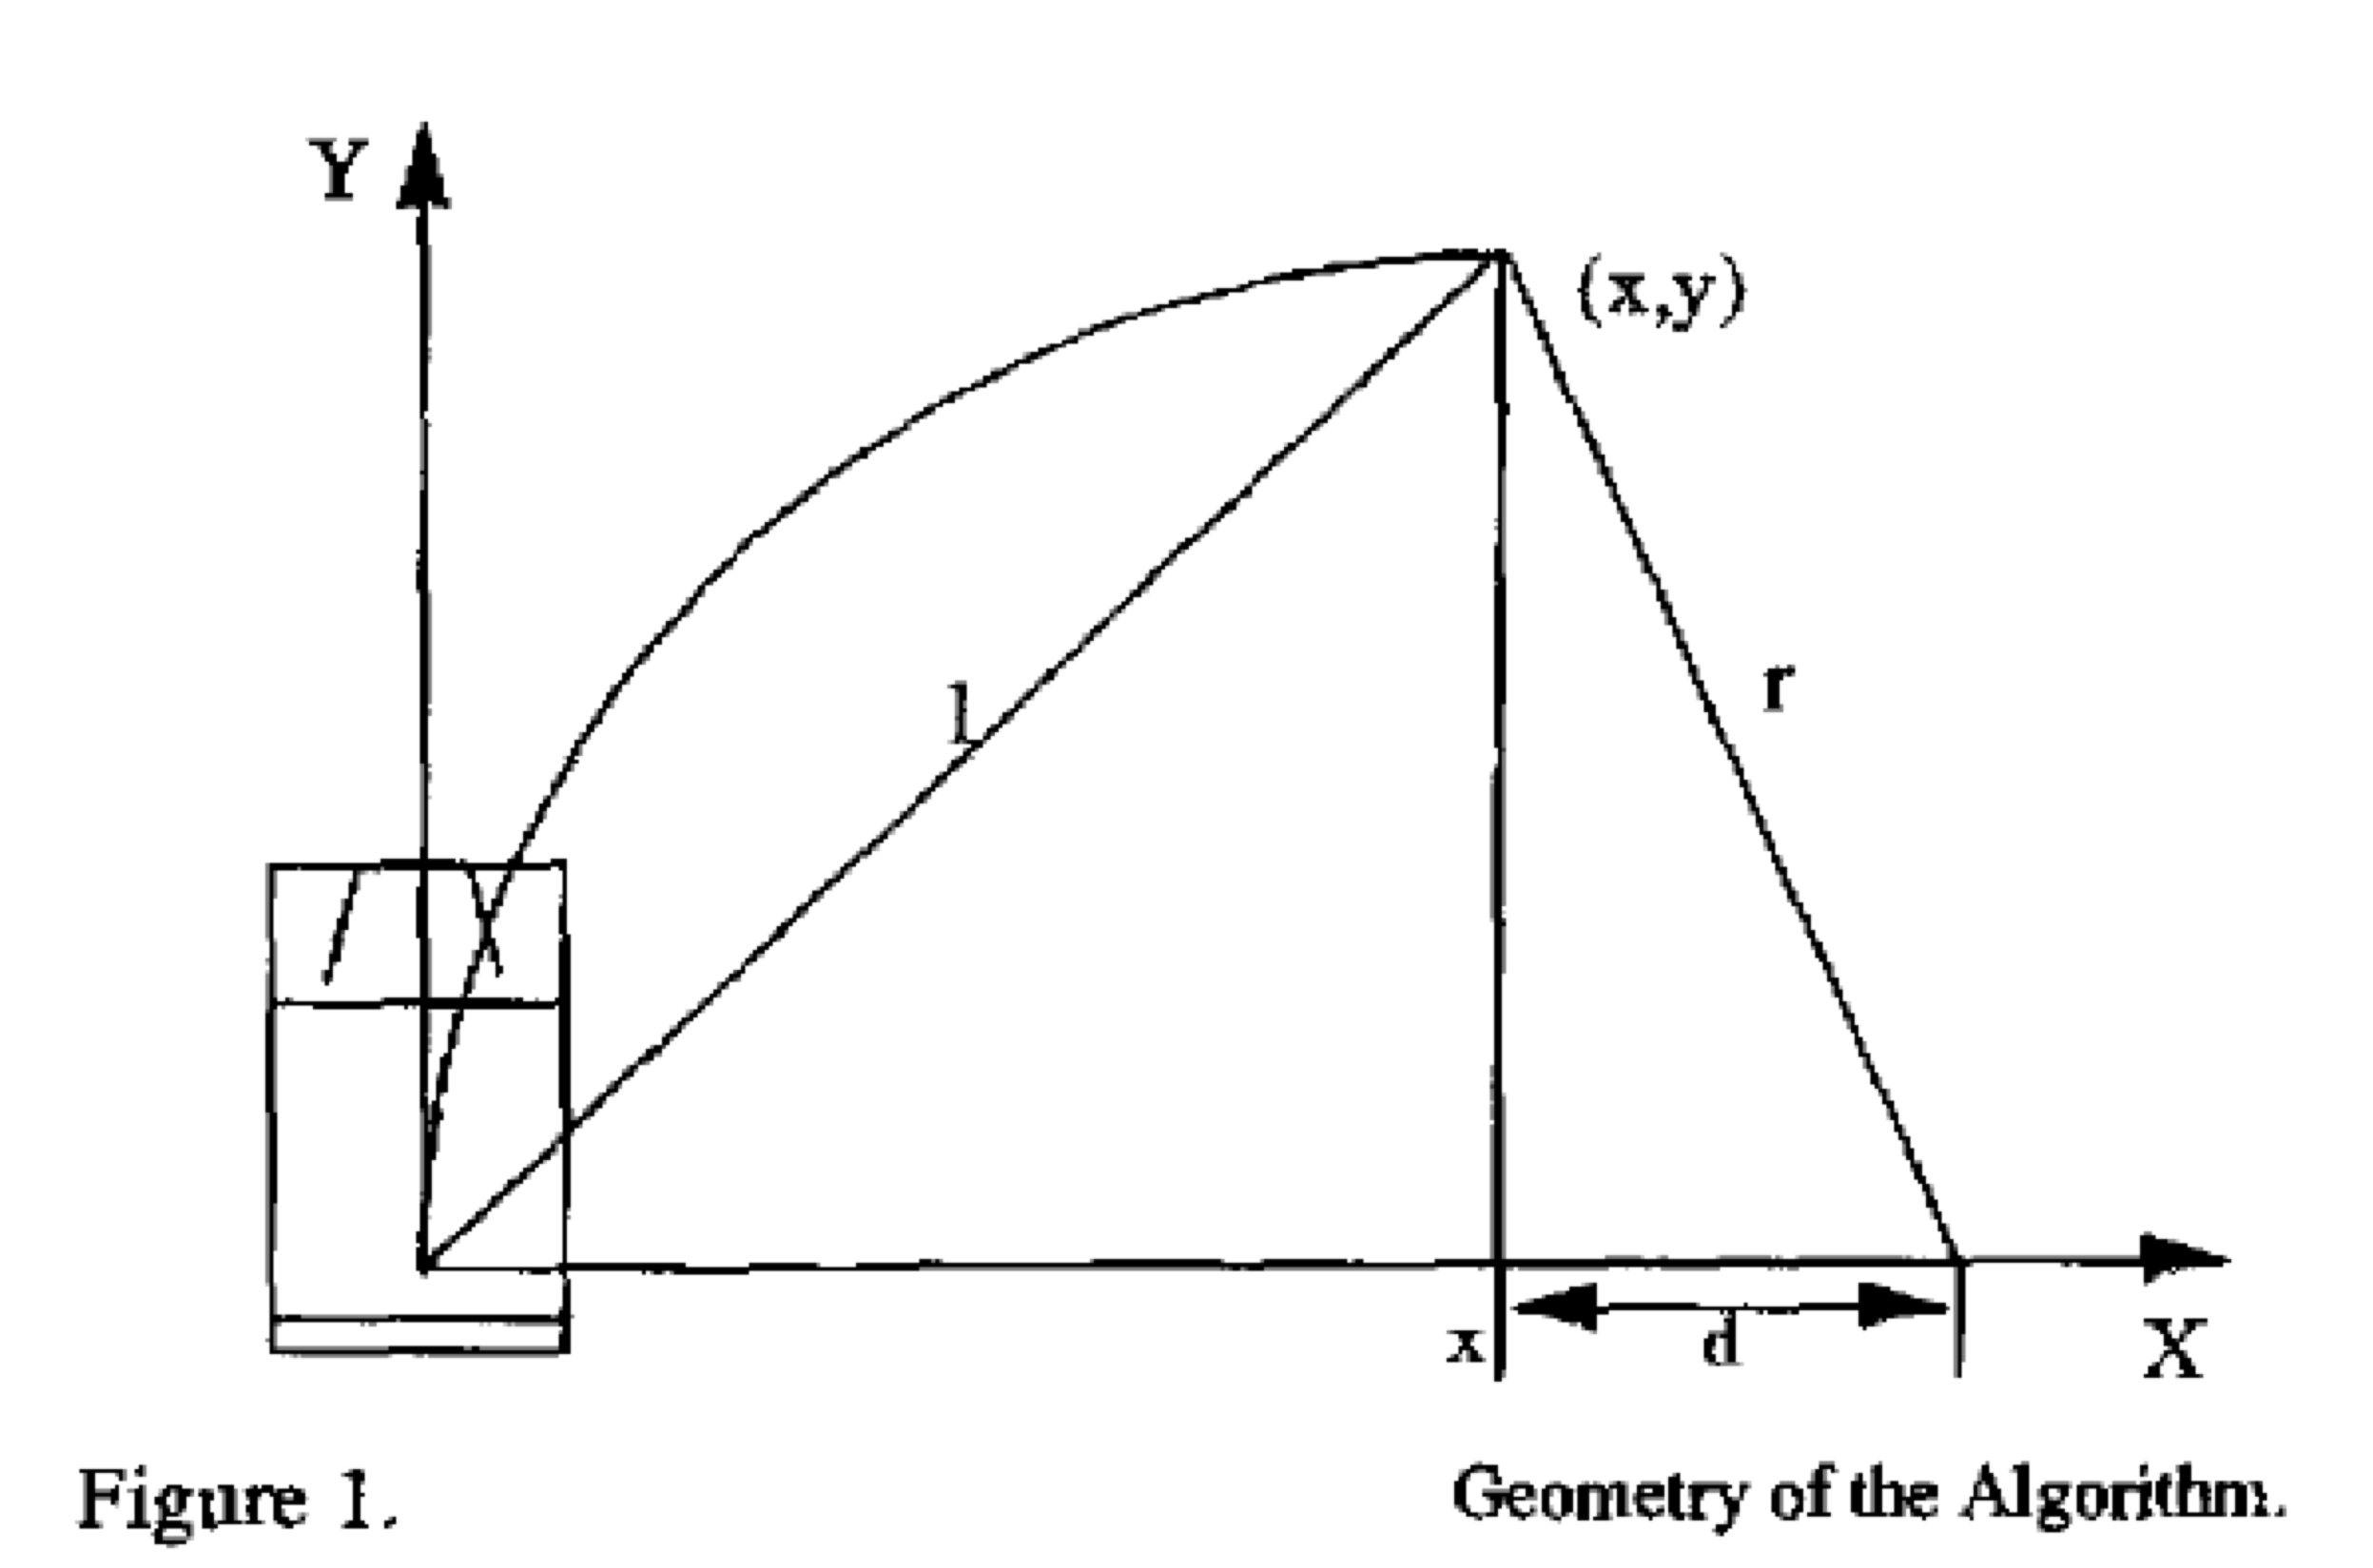
\includegraphics[scale=.5]{figures/pure_pursuit_geom}
	\caption{Geometry of Pure Pursuit Algorithm}
\end{figure}
\begin{align}
x^2+y^2=l^2\\
x+d=r
\end{align}

\noindent Now for the curvature such that:
\begin{align}
r=\frac{l^2}{2x}\\
\gamma=\frac{2x}{l^2}
\end{align}


\subsection{Behavioral Controller}
In \cite{Ninomiya} the authors develop a behavioral controller which mimics expert driving instructor behavior at blind corners. Specifically such drivers anticipate unseen obstacles and dangers. Such drivers should take different actions depending on their prediction of other potential traffic participants, including both pedestrians and vehicles. We allow that other traffic participants may not be within the sight of the test subject. As such the driver model is defined by three rules each of which produce an update to the vehicles acceleration: 
\begin{itemize}
	\item If a potential (even unseen) traffic participant is likely to collide, the driver will brake proactively, 
	\item else if the current speed is below a desired speed, accelerate, 
	\item otherwise, keep the current speed. 
\end{itemize}

Assuming that the ego vehicle and a potential traffic participant are point masses and will cross perpendicularly, we will model the above rules by acceleration of the ego vehicle:

\begin{equation}
y_{ot}+v_{ot}t_c < \frac{w}{2} \to a_{et} = \frac{v_{et}^2 - v_{min}^2}{2(x_{et}-x_{min})} 
\end{equation} 
\todo[inline]{looks like the ego accelerates (positive acceleration) even though there's an impending collision?}
\begin{equation}
v_{et}<v_d \to a_{et}=	\frac{v_{d}^2 -v_{et}^2}{2(x_d - x_{et})}
\end{equation}

\noindent Otherwise...
\begin{equation}
a_{et}=0
\end{equation}
Here, $(x_{et}, y_{et}, v_{et})$,$(x_{ot}, y_{ot}, v_{ot})$, $(x_d,v_d)$ are the position and speed of ego vehicle at time t, the current position and speed of a potential traffic participant at time t, and the desired final state of the ego vehicle, respectively. $(x_{min},v_{min})$  is the state (position and speed) after finishing deceleration. By introducing a minimum admissible displacement $\epsilon$ , $x_{min}$  can be expressed as
\begin{equation}
x_{min} - x_0=\epsilon
\end{equation}


Where $t_c$  is a predicted time to collision derived as a function of the speed of the ego-vehicle:
\begin{equation}
t_c=max(\frac{x_{ot}-x_{et}}{v_{et}},0)
\end{equation}

Thus, the condition $y_{ot}+v_{ot}t_c < \frac{w}{2}$  means that the trajectory of the potential traffic participant will reach and stay within a set in which collision is possible $w$, at the time to collision. We assume that the potential traffic participants begin their paths behind a wall in the occluded region on the left of the intersection.\\
\textbf{This changes... because we will add differential inclusions}\\
Each traffic participant may move at a constant speed, from left to right in the scene. This is a reasonable assumption because the side road restricts vehicles to drive one way. Given the wall position $(x_w,y_w)$, the position $(x_{ot},y_{ot})$  are expressed as
\begin{equation}
x_{ot}=\gamma d + x_{w}
\end{equation}
\begin{equation}
y_{ot} = \gamma d + (x_w - x_{et})tan(\rho_t) +y_{et}
\end{equation}

Here, $d$ is the width of the side road and $\rho_t$ is the current field of view from the ego vehicle driver computed as:
\begin{equation}
tan(\rho_t) = \frac{y_w-y_{et}}{x_w - x_{et}}
\end{equation}

Note that   is a parameter defining the x position of a potential traffic participant that takes a value from 0 to 1. From equations (1) to (9), one can compute a desired speed profile and trajectory with which the driver can avoid collision to a potential traffic participant coming out from the position $(x_{ot},y_{ot})$ at speed $v_o$.


\noindent \textbf{Traffic Control}
\begin{itemize}
	\item Stop Sign
	\item Speed Limit
	\item Yield
	\item Traffic Light
\end{itemize}

\noindent \textbf{Pedestrians}
\begin{itemize}
	\item Dynamics
	\item Grid based abstraction
	\item Non determinism
\end{itemize}

%------------------------------------------------------------------------------
\section{Benchmarks}
\subsection{A Simple Lane Change}
\begin{itemize}
	\item We first present this scenario in \cite{blah}
	\item Other authors \cite{blah} have considered with static obstacles
	\item Counterexamples are somewhat obvious
	\item Inductive invariance argument allows verification of infinite time properties
		\item Most examples involving forward safety are monotonic ie selecting a lower operating speed implies an decrease in stopping time and improves the forward safety of the vehicle. 
		\item In such problems there are no ``holes" in the interval. 
		\item Resulting proofs seem to indicate that testing would be sufficient to find counterexamples because unsafe results occur at extreme points in the state space only.
		\begin{itemize}
			\item Verification still provides a guarantee of safety that was not previously available. 
			\item Verification is still useful for formally verifying specifications and interaction between supplier systems and vehicle dynamics.
			\item Helps to search for viable combinations of specifications
		\end{itemize}
	\item We extend this scenario with differential inclusions. 
	\item Problem: we are forced into the tree representation because we cannot bring the trajectory generator in the dReach framework, requires external libraries and iteration. Could be remedied via creation of a lookup table or Neural Network. Alternative is to change the trajectory generation strategy such as Pure Pursuit.
\end{itemize}

\subsection{Algorithm}
How we establish safety of a decision controller.
\begin{algorithm}
	\caption{Check Trajectory Sequence}
	\label{algo:trajseq}
	\begin{algorithmic}
		\State \textbf{checkSequence} (searchDepth)
		\State  bool $safetyVar := TRUE$
		\State int $depth := 0$
		\While {$depth \leq searchDepth$}
		\State float* $trajectoryParam = getNextTrajectory(depth)$
		\State $safetyVar := checkTrajectory(trajectoryParam)$
		\State
		\EndWhile
		\State \Return {$safetyVar$}
	\end{algorithmic}
\end{algorithm}
Proofs and lemmas:
\begin{itemize}
	\item Proof of compositional nature of safety of sequence of trajectories
	\item Assume gurantee reasoning for parallelization of verification procedure
	\item Inductive invariance for search termination at a specified depth. 
\end{itemize}

\begin{theorem}
	Proof of compositional nature of safety of sequence of trajectories
\end{theorem}

\begin{theorem}
	Contract for parallel composition of verification instances
\end{theorem}

\begin{theorem}
	Inductive invariance for search termination at a specified depth. 
\end{theorem}


\subsection{Variations in Road Geometry}
%\textbf{Random Ideas, not to be taken seriously}
%\begin{itemize}
%	\item Can we think of a type theoretic description of configuration space rather than set theoretic?
%	\item For example think of configuration space as a type
%	\item Pose and Goal can then be considered points of the configuration space type 
%	\item There exists many paths between a single pose and goal pair, all of these paths are equivalent from a type theoretic perspective.
	%\item Narrow down an instance of these paths by describing a decision procedure necessary to generate the path ie pure pursuit or cubic splines, the type of these functions is a path between goal and pose. 
%\end{itemize}

\begin{itemize}
	\item In order to pursue more complex scenarios with more expressive agents we propose a variation in the trajectory generation strategy which admits a closed form
	\item Implement pure pursuit trajectory generation strategy...
\end{itemize}
\begin{itemize}

	\item Open question if we can guarantee infinite time properties in general case, or on road by road basis via inductive invariant. 
	\item A second question of interest is the scalability of results involving multiple agents and curved roads. 
	\item Pure Pursuit can be represented directly in the Hybrid Program and admits a closed form solution for curvature.
	\item Using a Hybrid program we now show how the number of paths through the state space grows exponentially with the addition of other agents and events as well as increases in search depth. 
\end{itemize}

We present a scenario as shown in Figure \ref{fig:scenario2}
\begin{figure}
	\centering
	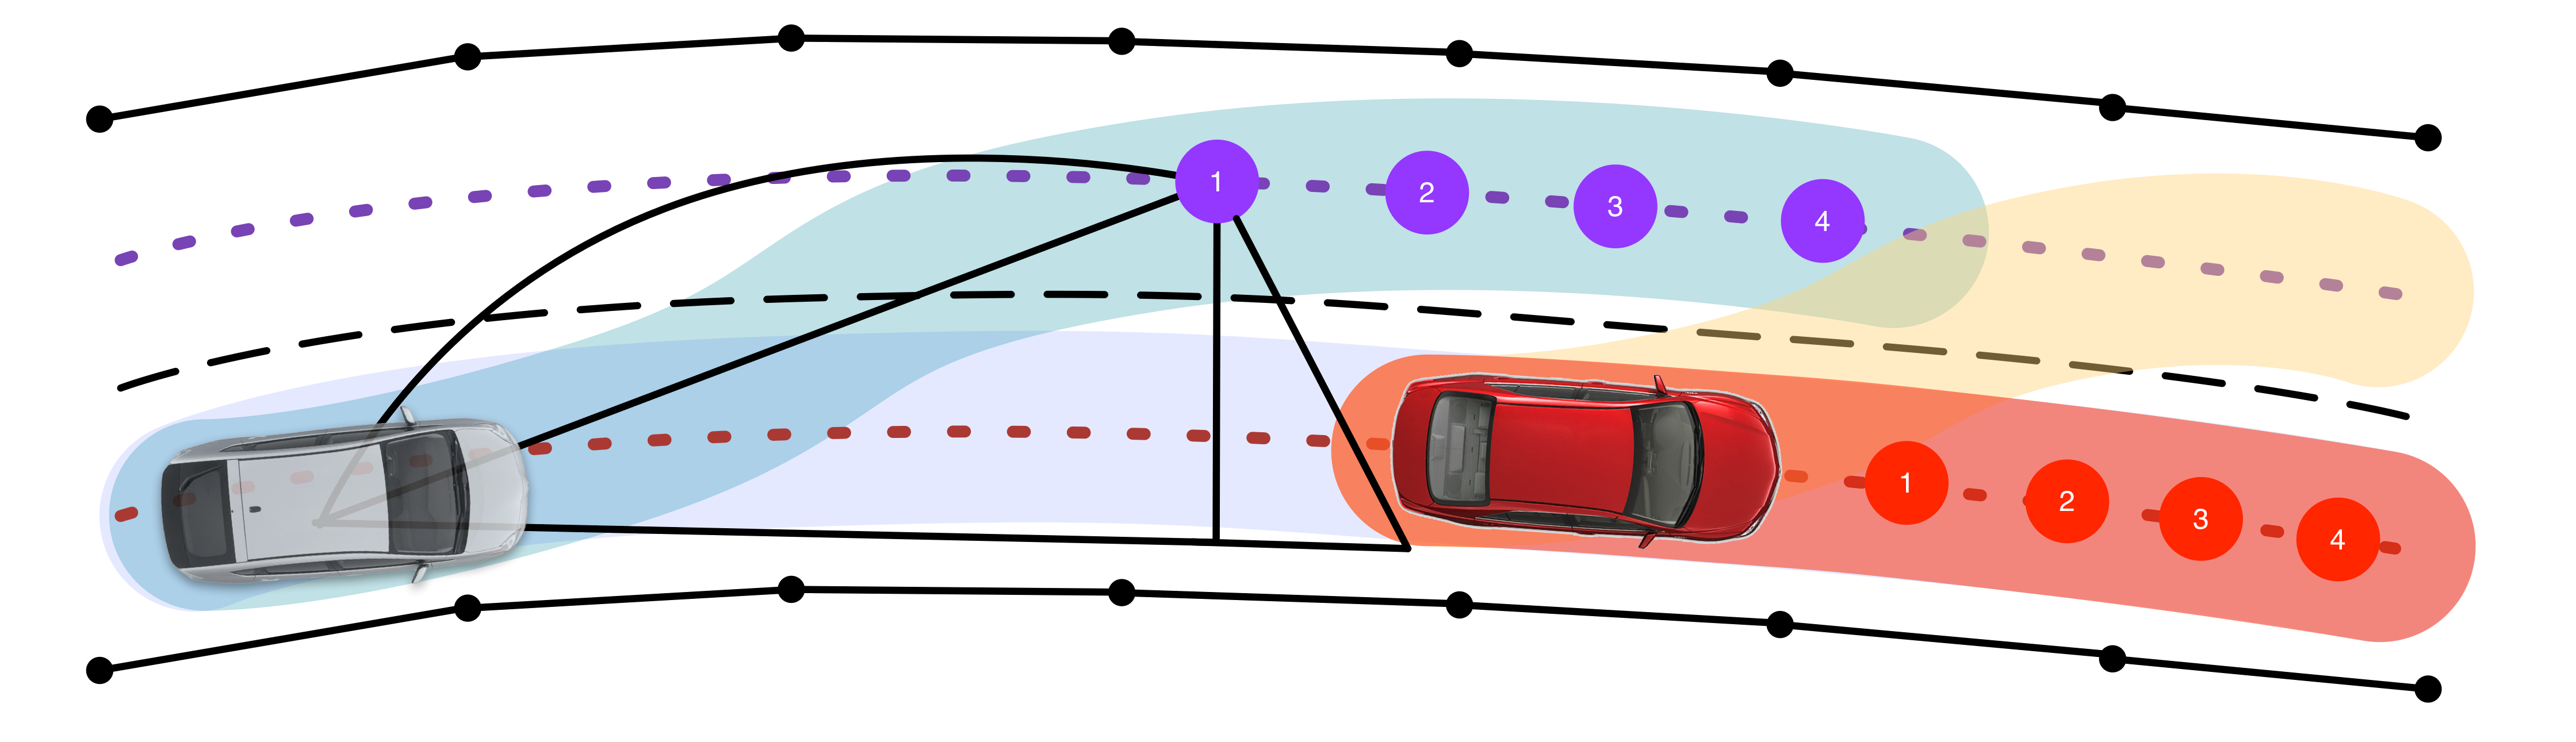
\includegraphics[scale=.4]{figures/scenario2}
	\caption{A graphical representation of the lane change scenario on a curved road}
\end{figure}
\begin{itemize}
	\item The previous example is the simplest possible instantiation of a lane change scenario
	\item Here we present an increasingly nuanced view of the the vehicle environment system
	\begin{itemize}
		\item Singleton inital sets and deterministic transitions
		\item Initial sets defined by intervals
		\item Non-determinism as applied to discrete decisions by the environment
		\item Automaton complexity in terms of states as number of agents grows
		\item Automaton complexity in terms of states as number of reference trajectories grows
		\item Search complexity in terms of path length as number of agents grows
		\item Search complexity in terms of path length as number of reference trajectories grows
		\item Non-deterministic scheduling of trajectory update
		\item Environment agents continuous dynamics are represented as differential inclusions (another form of non-determinism)
		\item Ego vehicle agents continuous dynamics are disturbed via errors represented as differntial inclusions
		\item Ego vehicle and environmental agents subjected to discrete events representing sensor or actuator failures.
	\end{itemize}
\end{itemize}
%Here we present a toy problem which explains why testing and monotonicity arguments might fail. This example was first presented in \cite{blah blah}.
%\begin{figure}[h]
%	\centering
%	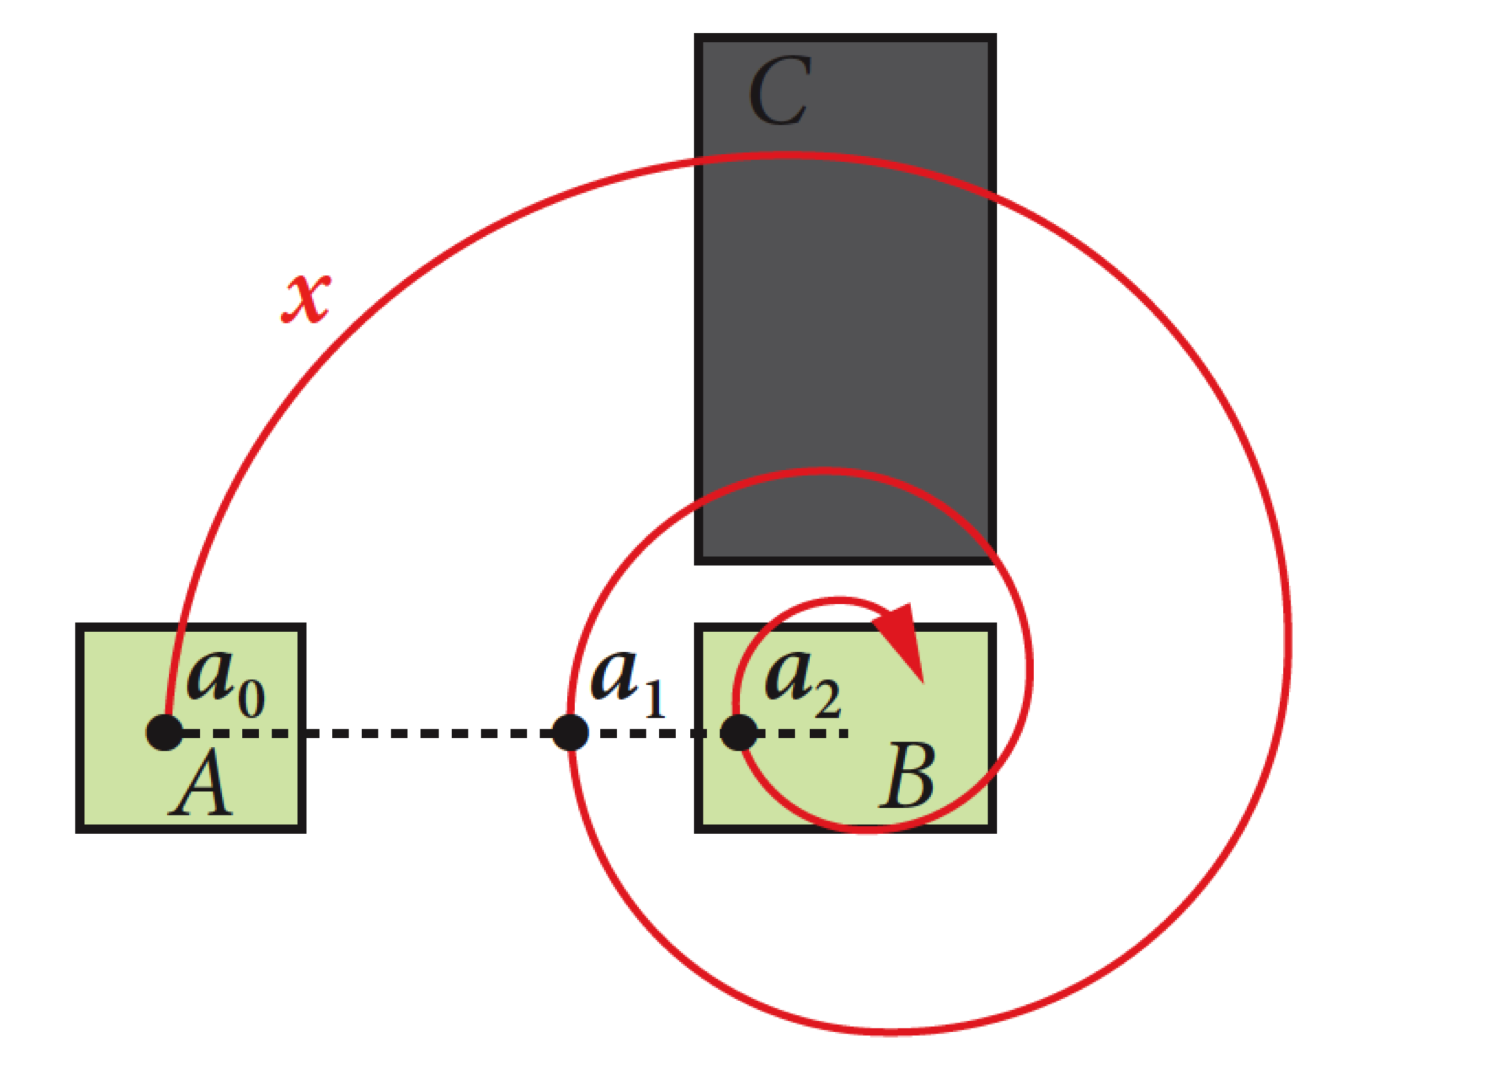
\includegraphics[scale=.4]{figures/diunsafe.png}
%	\caption{An example of a reach avoid problem with non-trivial counterexample}
%\end{figure}


\subsection{Proactive Expert Driver Assistance}
\textbf{Copy Paste from Nagoya stuff I wrote over summer, must be changed later...}\\
In many driving scenarios, the ego-vehicle must anticipate both visible and invisible dangers in the surrounding environment in order to plan safer paths. In residential areas, pedestrians and other vehicles are often completely occluded. In order to reduce the number of severe traffic accidents, proactive driving and pro-active driver models for unseen dangers are important next steps.

Proactive driver models are differentiated from emergency braking systems such as pre-crash safety which react to (1) dangers already in sight, (2) longer-range phenomena still measurable by sensors, (3) or detailed knowledge of road infrastructure. Instead proactive driver models and ADAS must deal with a predicted level of danger in current traffic conditions as an input to the model. 

For example, while passing through intersections with a blind corner, the proactive driver model would decelerate in relation to a prediction of the state of other traffic participants, even those which have not yet been sensed. We note, however, that the state space of the other traffic participants contains an infinite number of possible configurations and a large (but finite) number of scenarios, complicating proactive driver model construction. Although attempts have been made to develop controllers, which anticipate hazards in a blind area, the computational principals governing the design and safety of such a system are not yet clear. 

In previous works as first step towards creating data-driven proactive ADAS is to understand the behavior of a variety of human drivers. Thus, we collected and analyzed driving data on a public road where drivers need to anticipate unseen dangers. Tests included driving in a residential area, performed by both expert and elderly subjects and accurately analyzed by means of a high-precision data acquisition system. 

%------------------------------------------------------------------------------

%------------------------------------------------------------------------------

%------------------------------------------------------------------------------


\section{Conclusions}

	\begin{itemize}
		\item Types of Uncertainty:
		\begin{itemize}
			\item Scenario Configuration
			\item Initial Estimation Errors
			\item Noise in dynamics
			\item Sensor estimation errors
			\item Sensing thresholds
		\end{itemize}
	\end{itemize}
	\begin{itemize}
		\item Scenario 1: Lane change on straight road with two agents
		
		\item Scenario 2: Curved road with hybrid program representation
		\begin{itemize}
			\item No longer have clear invariant cut
		\end{itemize}
		\item Scenario 3: Obstructed T-Junction
		\begin{itemize}
			\item Map provides knowledge of obstruction and automatically adjusts behavior
		\end{itemize}
		\begin{itemize}
			\item Variant: Traffic light
			\item Variant: Pedestrian
		\end{itemize}
	\end{itemize}


\label{sect:bib}
\bibliographystyle{plain}
%\bibliographystyle{alpha}
%\bibliographystyle{unsrt}
%\bibliographystyle{abbrv}
\bibliography{easychair}

\begin{comment}
%------------------------------------------------------------------------------
\appendix
\section{Formatting Information}
\label{sect:easychair-requirements}
\begin{enumerate}
	\item
	The default paper size is US letter. It can be explicitly set to A4 
	(\texttt{a4paper}) or letter (\texttt{letterpaper}) paper in the
	document class entry, e.g.:\\\verb+\documentclass[a4paper]{easychair}+
	
	\item
	The print area for both letter and A4 paper sizes is 145x224 mm. This size
	has been selected to allow for inexpensive printing using our current
	print-on-demand publisher.
	
	\item
	The base font is Computer Modern. The base font size is 10pt. If you
	use any other font size, there is no guarantee that the produced
	document will look nice or fit into our standard page size.
	
	\item
	The references list is condensed. The default bibliography styles, such as
	\texttt{plain}, \texttt{abbrv}, and \texttt{alpha}, are suggested.
	
	\item
	PNG, JPG, and PDF images are supported, i.e., those that are supported
	by the standard \texttt{graphicx} package \cite{graphicx-package}, and
	render nicely in online versions of PDF documents.  This document
	shows some examples of JPG and PDF images, for example in
	Figure~\ref{fig:easychair-logo}. If the papers are designed for
	publishing in print, the images should be at least 300dpi in
	resolution. 
	
\end{enumerate}

\subsection{Tables}

Many page overflows happen because of large tables. In many case these
overflows can be easily removed by slightly reducing padding added by
\LaTeX\ to every column. It is controlled by the \LaTeX\ command
\verb|\tabcolsep| whose value by default is 6pt. Even small changes in
the value of this command may give drastic reductions in the width of
tables. This is illustrated in Figure~\ref{fig:tabcolsep} on
page~\pageref{fig:tabcolsep}. Note though that there is no free lunch:
smaller values for this command may result in lower redability.

%------------------------------------------------------------
\begin{figure}[tb]\small
	\begin{center}
		\begin{tabular}{lrrrrrrrr}
			\hline
			ATP System            & LTB & Avg  &Prfs & SOTA & \multicolumn{1}{c}{$\mu$} & CYC & MZR & SMO \\
			\hline
			Vampire-LTB 11.0      &  69 & 24.5 &  69 & 0.37 & 28.1 &  23 &  22 &  24 \\
			iProver-SInE 0.7      &  67 & 76.5 &   0 & 0.36 &  8.8 &  28 &  14 &  25 \\
			\hline
		\end{tabular}
	\end{center}
	
	\begin{center}\renewcommand{\tabcolsep}{5pt}
		\begin{tabular}{lrrrrrrrr}
			\hline
			ATP System            & LTB & Avg  &Prfs & SOTA & \multicolumn{1}{c}{$\mu$} & CYC & MZR & SMO \\
			\hline
			Vampire-LTB 11.0      &  69 & 24.5 &  69 & 0.37 & 28.1 &  23 &  22 &  24 \\
			iProver-SInE 0.7      &  67 & 76.5 &   0 & 0.36 &  8.8 &  28 &  14 &  25 \\
			\hline
		\end{tabular}
	\end{center}
	
	\begin{center}\renewcommand{\tabcolsep}{3pt}
		\begin{tabular}{lrrrrrrrr}
			\hline
			ATP System            & LTB & Avg  &Prfs & SOTA & \multicolumn{1}{c}{$\mu$} & CYC & MZR & SMO \\
			\hline
			Vampire-LTB 11.0      &  69 & 24.5 &  69 & 0.37 & 28.1 &  23 &  22 &  24 \\
			iProver-SInE 0.7      &  67 & 76.5 &   0 & 0.36 &  8.8 &  28 &  14 &  25 \\
			\hline
		\end{tabular}
	\end{center}
	
	\begin{center}\renewcommand{\tabcolsep}{1pt}
		\begin{tabular}{lrrrrrrrr}
			\hline
			ATP System            & LTB & Avg  &Prfs & SOTA & \multicolumn{1}{c}{$\mu$} & CYC & MZR & SMO \\
			\hline
			Vampire-LTB 11.0      &  69 & 24.5 &  69 & 0.37 & 28.1 &  23 &  22 &  24 \\
			iProver-SInE 0.7      &  67 & 76.5 &   0 & 0.36 &  8.8 &  28 &  14 &  25 \\
			\hline
		\end{tabular}
	\end{center}
	\normalsize
	
	\caption{Original table and tables with \texttt{tabcolsep} set to 5pt,
		3pt, and 1pt
		\label{fig:tabcolsep}}
	
\end{figure}
%------------------------------------------------------------

\subsection{Images}

Images included using \verb|\includegraphics| are easy to resize since
one can specify the size of the result explicitly. For example,
Figure~\ref{fig:easythrone} shows three copies of the same image
having different sizes obtained using the following commands:

\begin{verbatim}
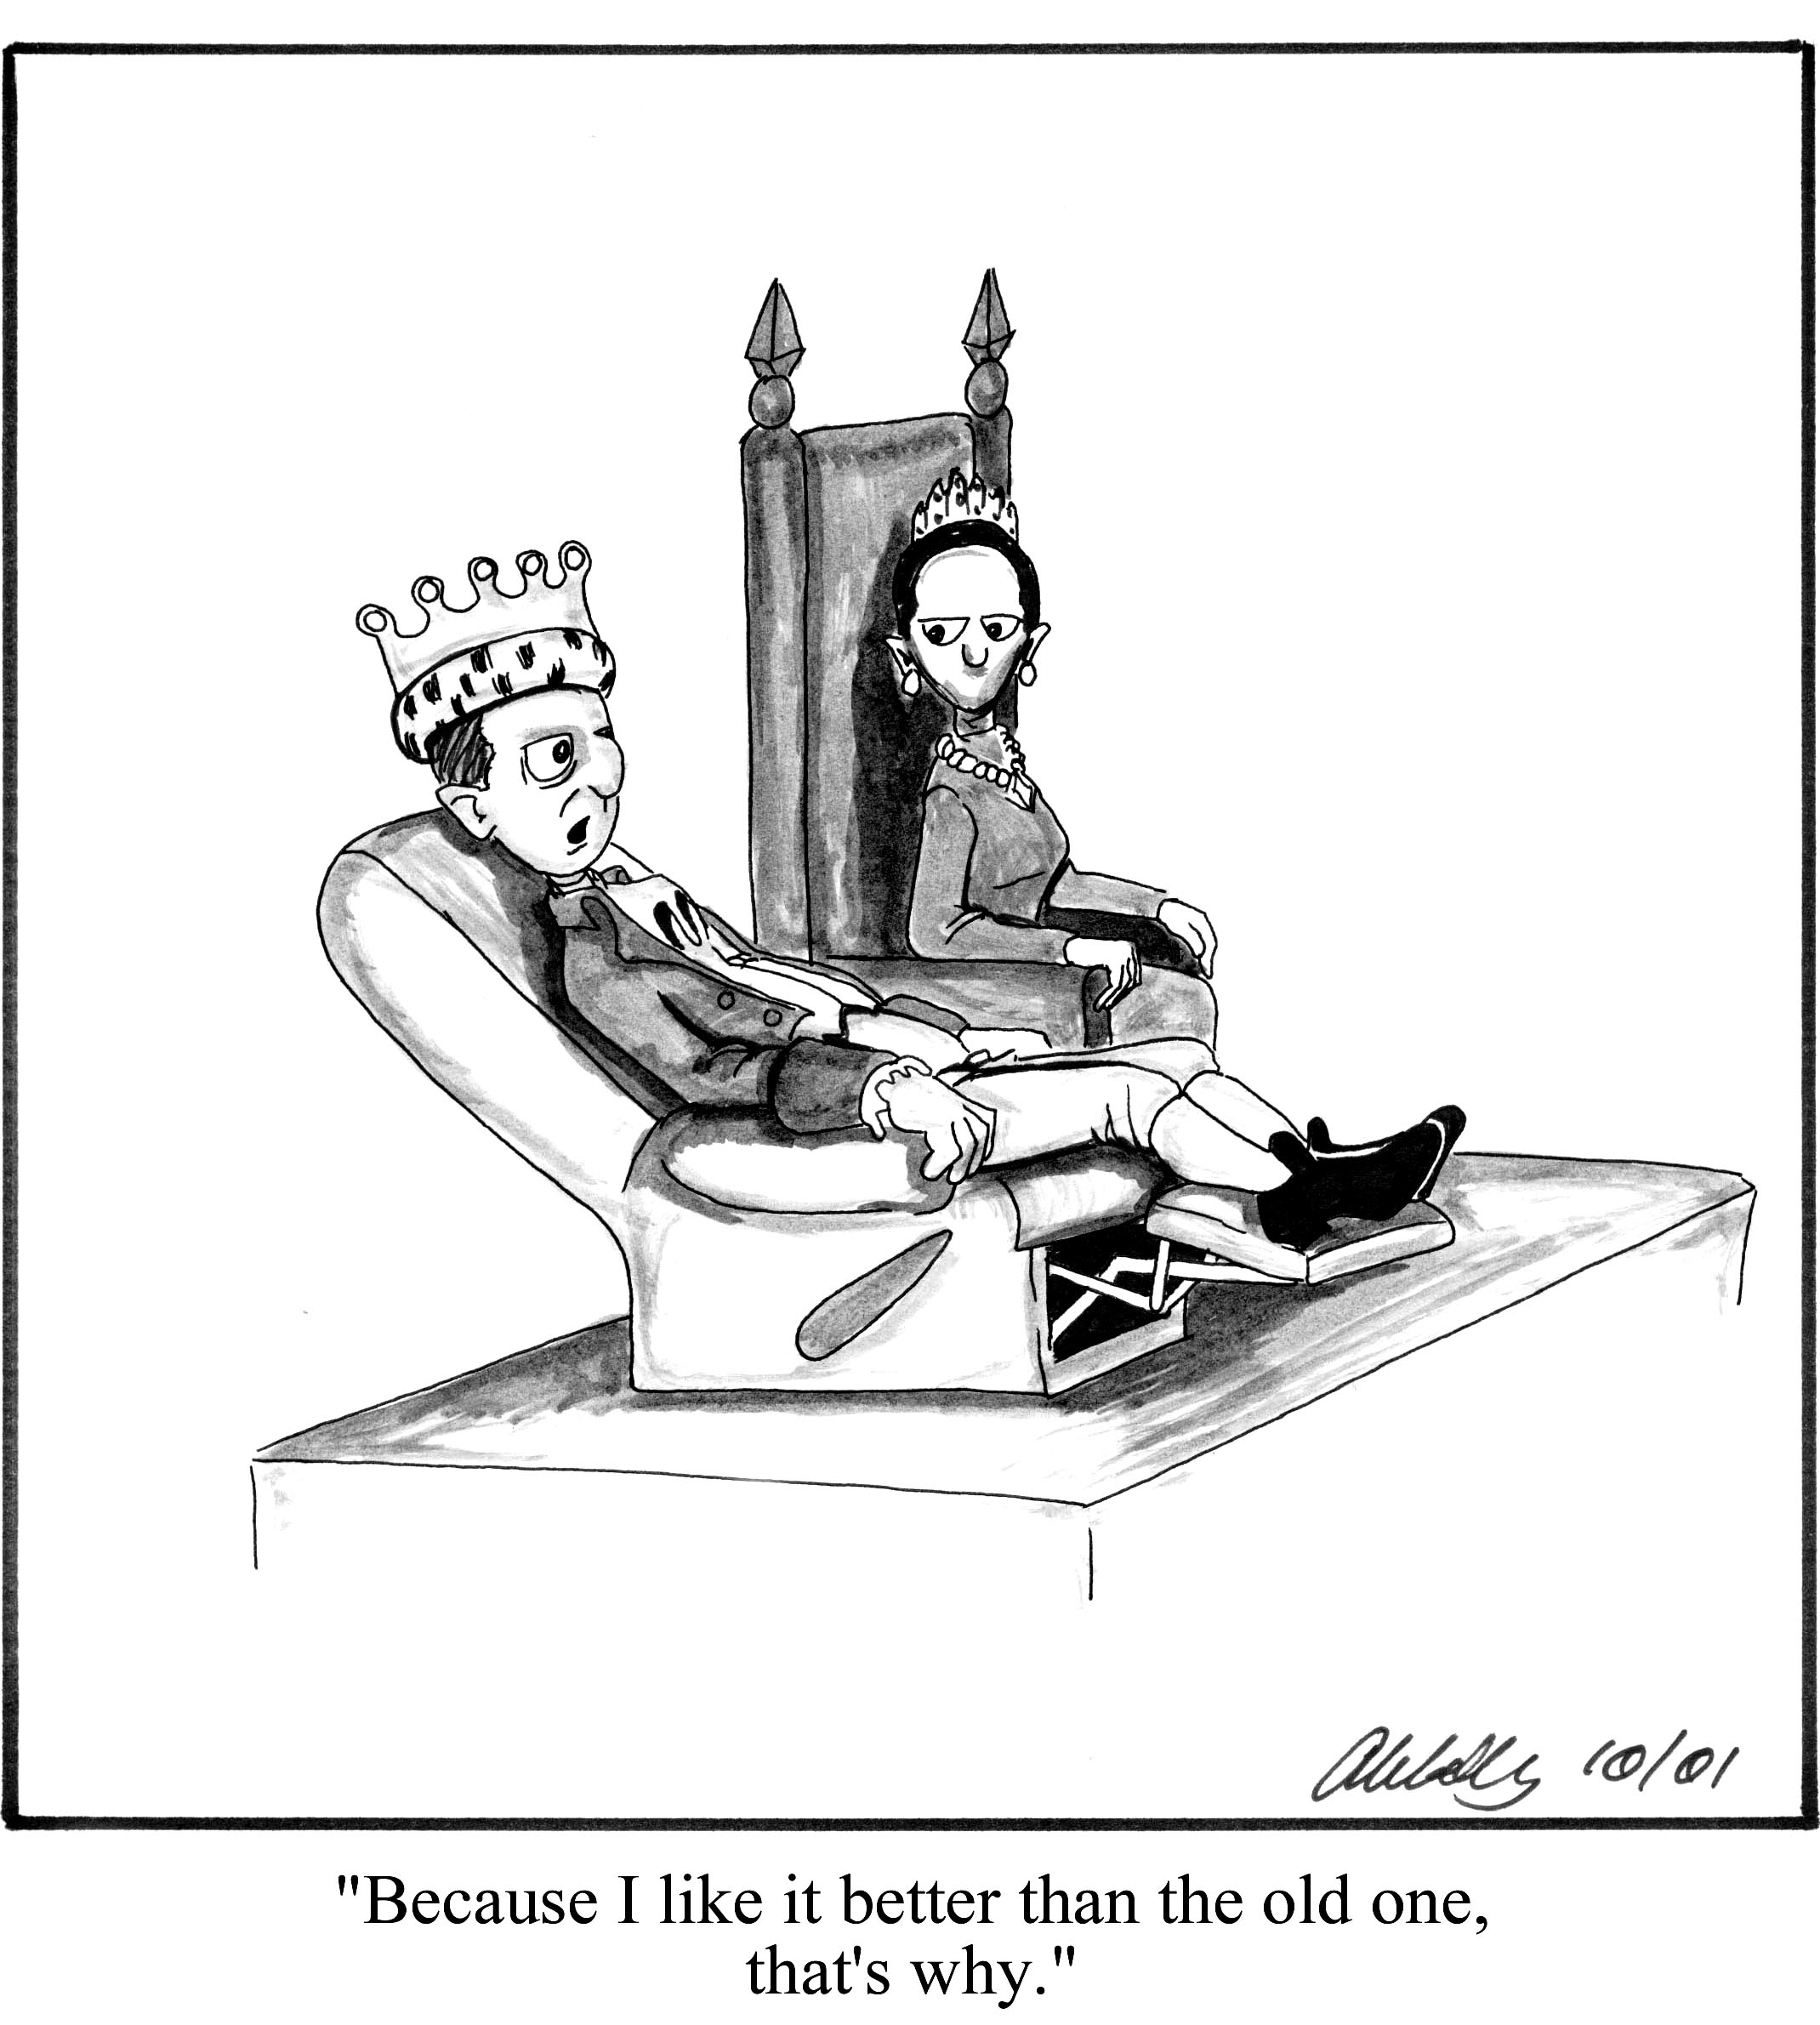
\includegraphics[width=0.5\textwidth]{throneEC.jpg}
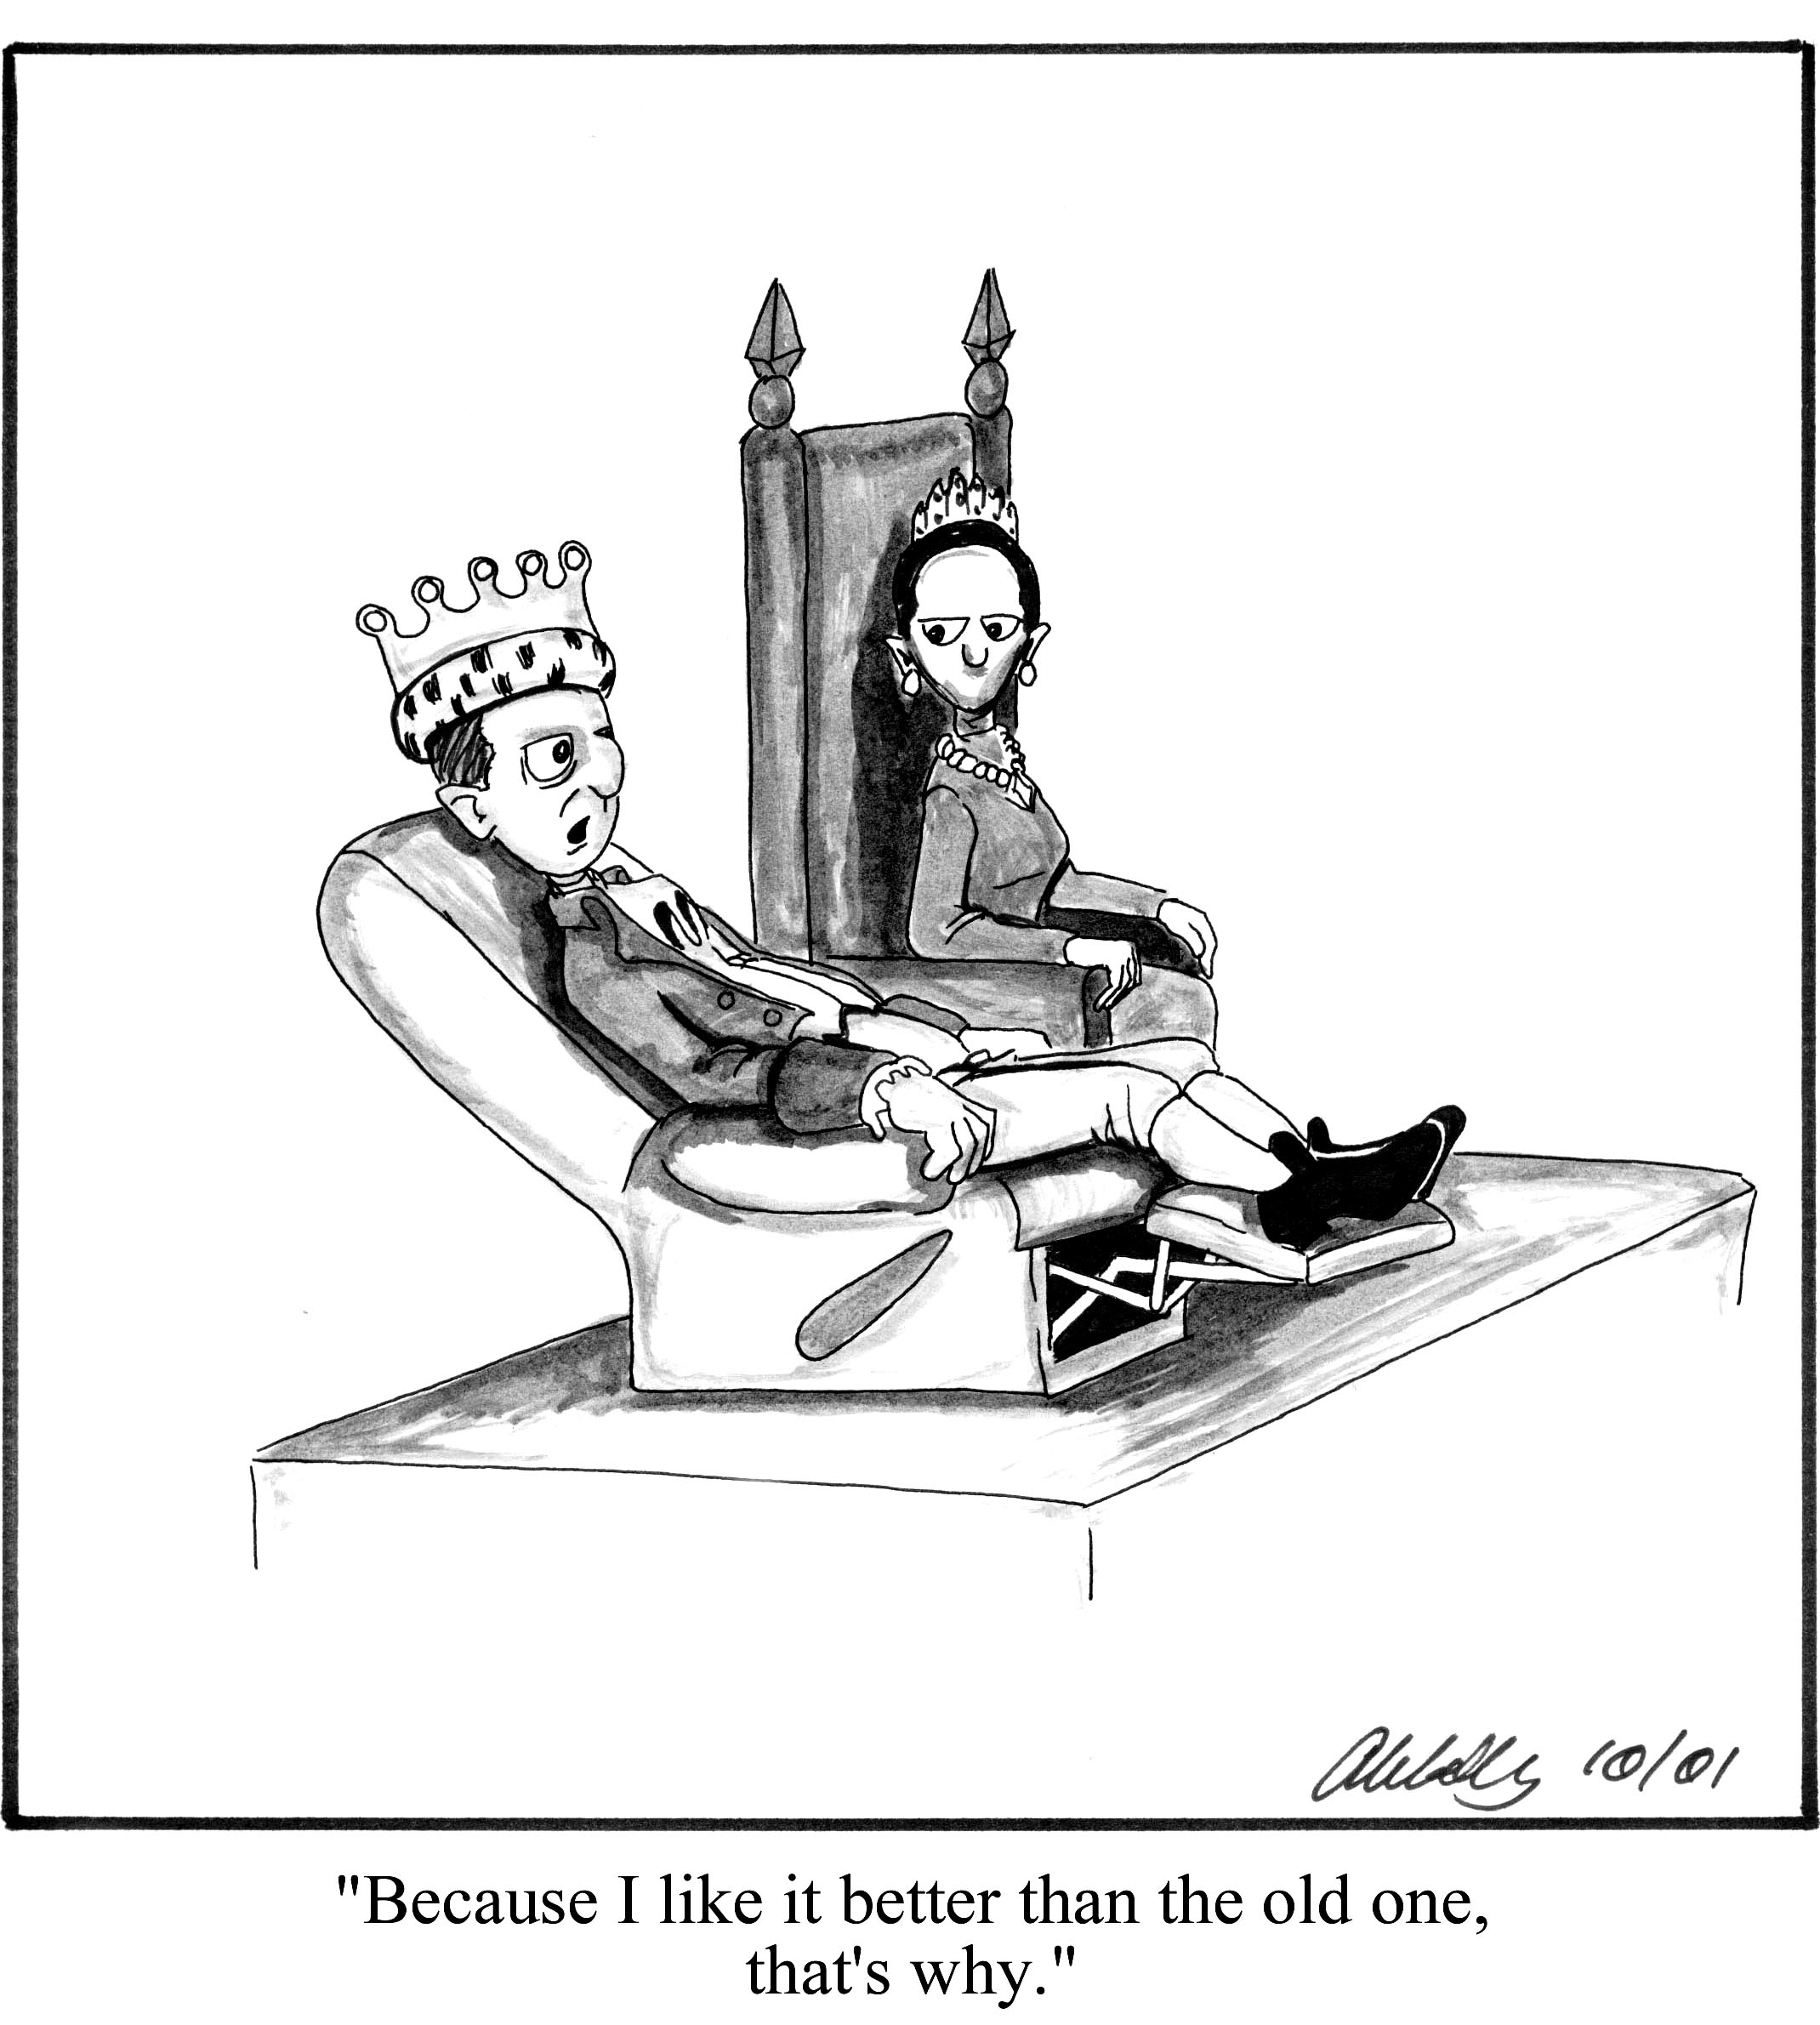
\includegraphics[width=0.3\textwidth]{throneEC.jpg}
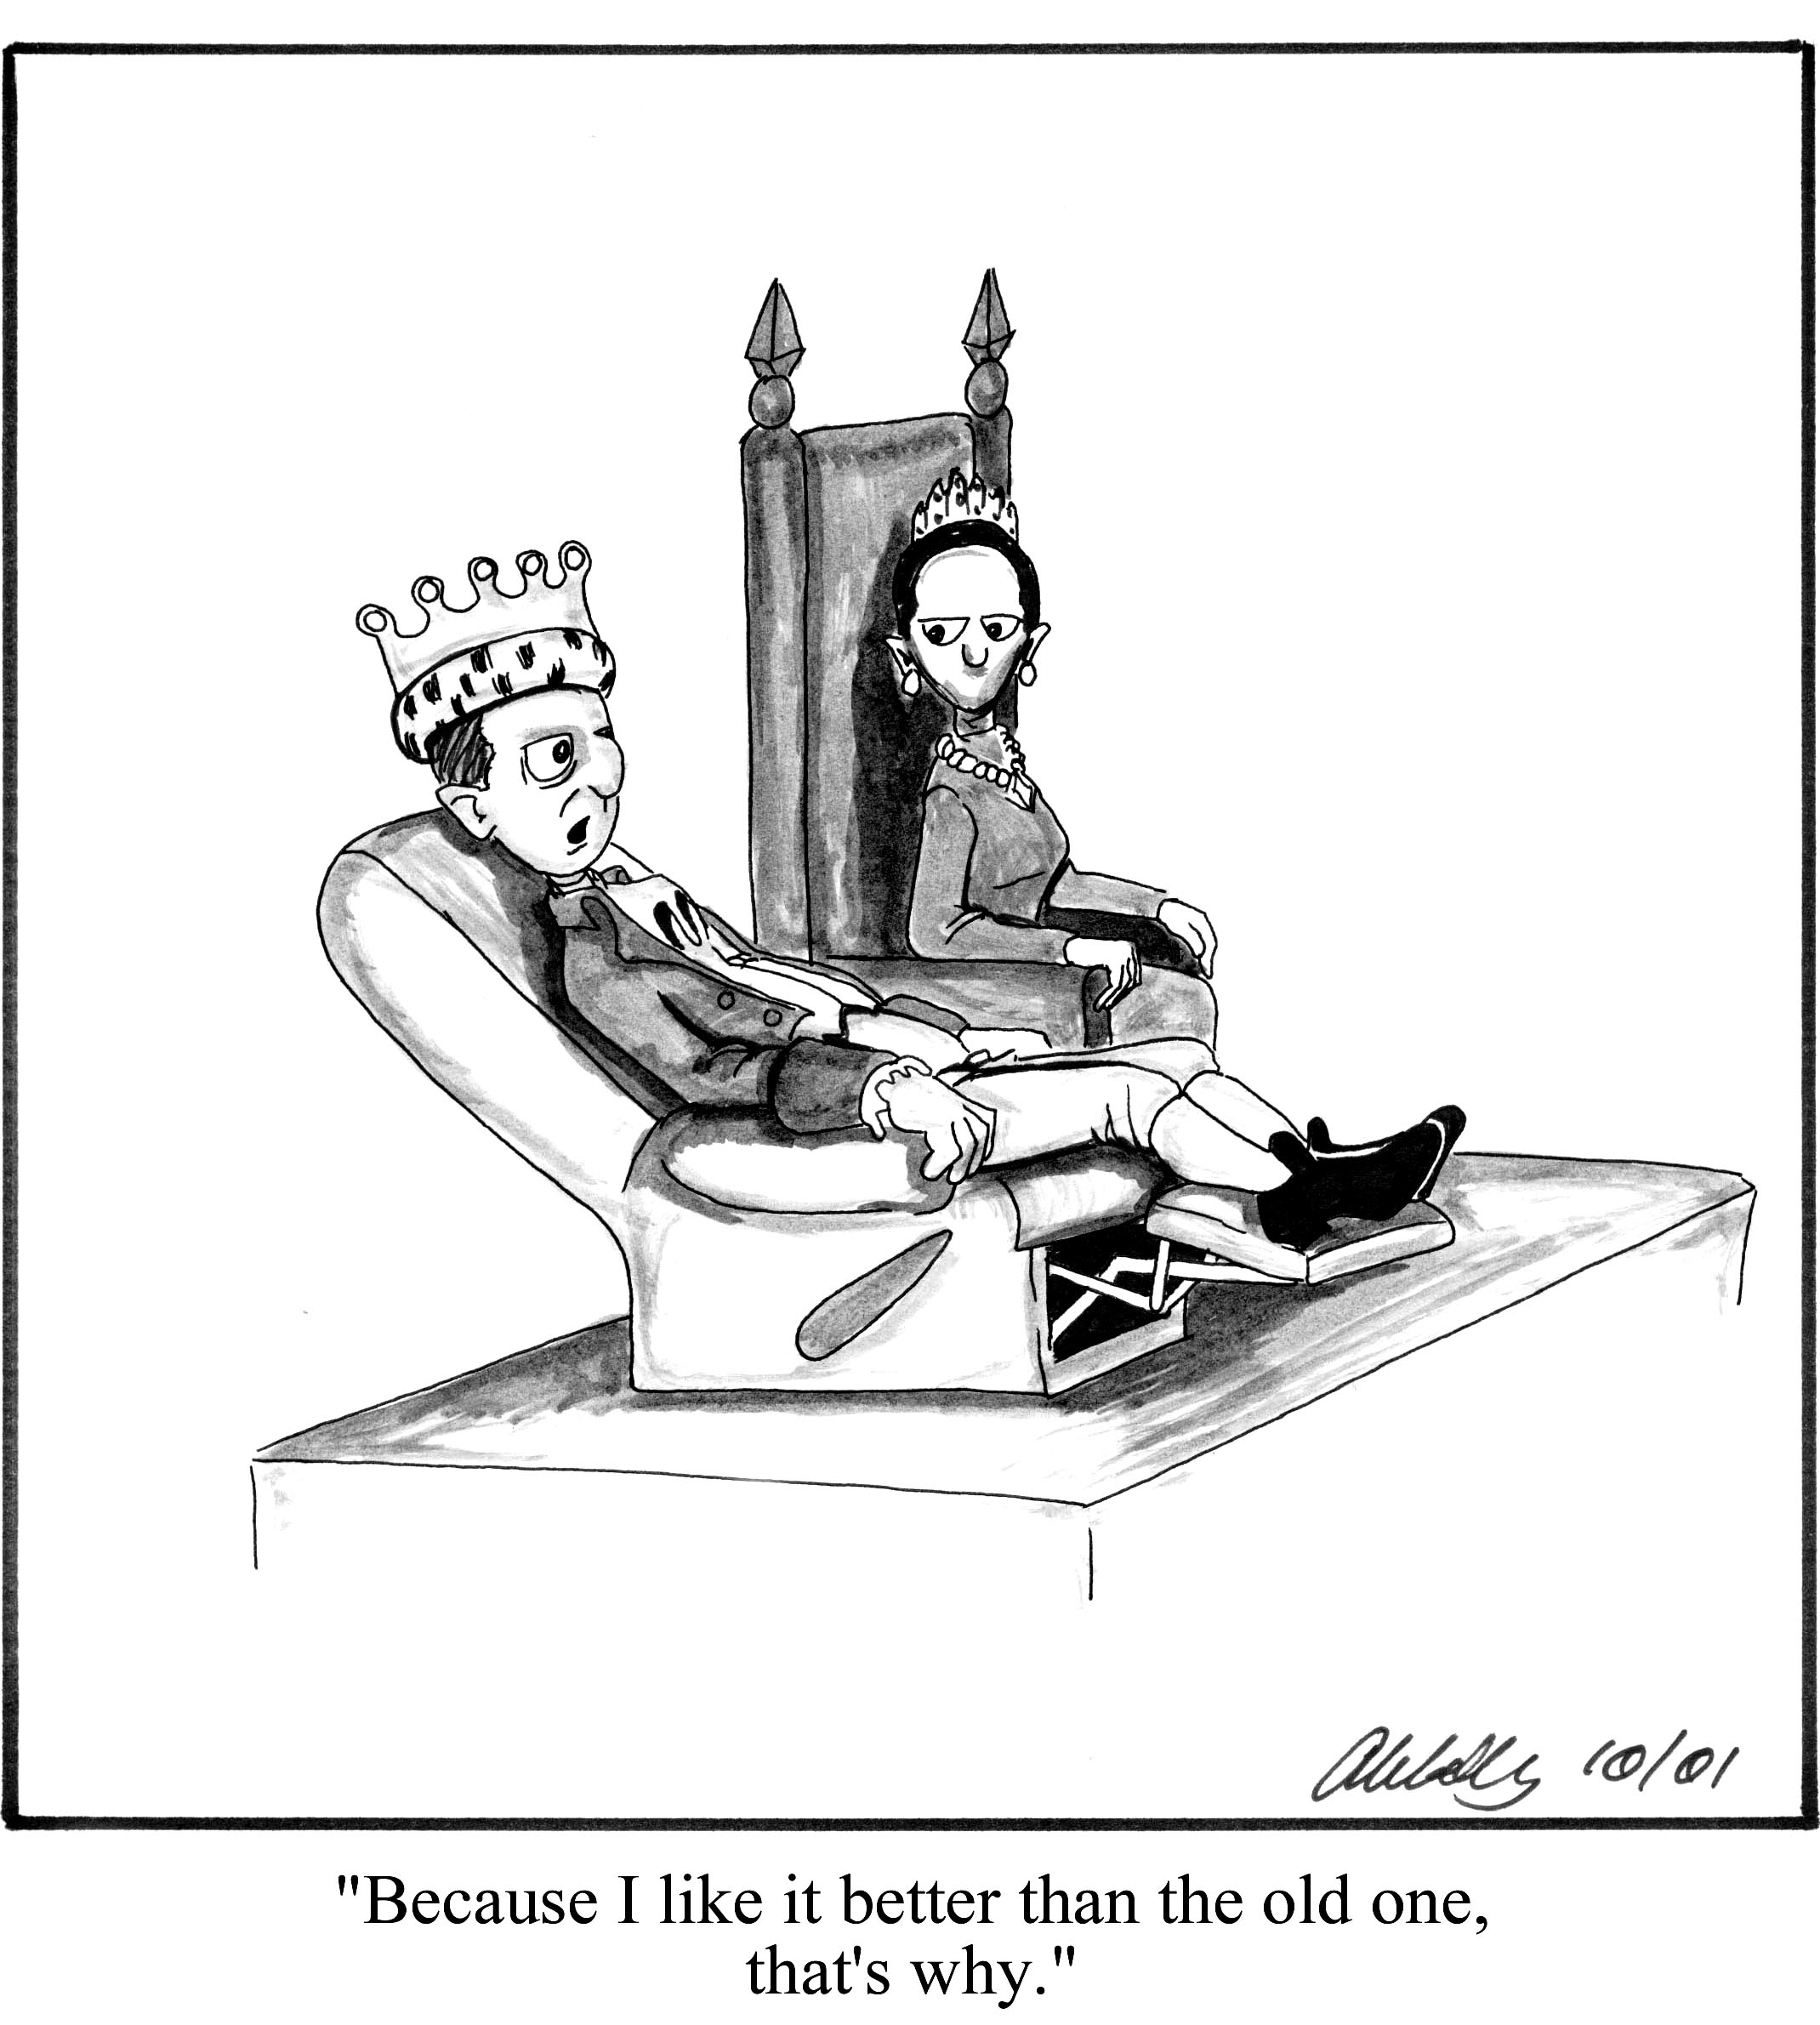
\includegraphics[width=0.15\textwidth]{throneEC.jpg}
\end{verbatim}

\subsection{A Universal Recipe}

\LaTeX\ has a very powerful weapon for reducing the size of almost
anythings. More precisely, it can reduce anything producing what
\LaTeX\ considers a box. This weapon is called
\verb|\scalebox|. Consider an example (check the source of this file
to see how it was produced).

\begin{center}
	\begin{tabular}{|c|c|}
		\hline \Huge
		\begin{tabular}[b]{cr}
			year & users \\ \hline
			2007 &    47,753 \\
			2008 &    114,494 \\
			2009 &    207,506 \\
			2010 &   371,054 \\
		\end{tabular}
		&
		
\includegraphics[width=0.28\textwidth]{chairEC}\\
		\hline
		\multicolumn{2}{|c|}{The number of users of EasyChair and one of its
			logos,}\\
		\multicolumn{2}{|c|}{scaled to the number of users in 2010} \\
		\hline
	\end{tabular}
\end{center}
This is what happens when we put (almost) the same \LaTeX\ code in 
\verb|\scalebox{0.55923}{...}| to scale it down to the number of users
in 2009:

\begin{center}
	\scalebox{0.55923}{%
		\begin{tabular}{|c|c|}
			\hline \Huge
			\begin{tabular}[b]{cr}
				year & users \\ \hline
				2007 &    47,753 \\
				2008 &    114,494 \\
				2009 &    207,506 \\
				2010 &   371,054 \\
			\end{tabular}
			&
			
\includegraphics[width=0.28\textwidth]{chairEC}\\
			\hline
			\multicolumn{2}{|c|}{The number of users of EasyChair and one of its
				logos,}\\
			\multicolumn{2}{|c|}{scaled to the number of users in 2009} \\
			\hline
		\end{tabular}}
	\end{center}
	We can scale it down even further to the 2008 figure using
	\verb|\scalebox{0.30856}{...}|:
	
	\begin{center}
		\scalebox{0.30856}{%
			\begin{tabular}{|c|c|}
				\hline \Huge
				\begin{tabular}[b]{cr}
					year & users \\ \hline
					2007 &    47,753 \\
					2008 &    114,494 \\
					2009 &    207,506 \\
					2010 &   371,054 \\
				\end{tabular}
				&
				
\includegraphics[width=0.28\textwidth]{chairEC}\\
				\hline
				\multicolumn{2}{|c|}{The number of users of EasyChair and one of its
					logos,}\\
				\multicolumn{2}{|c|}{scaled to the number of users in 2008} \\
				\hline
			\end{tabular}}
		\end{center}
		or further down to 2007:
		
		\begin{center}
			\scalebox{0.12870}{%
				\begin{tabular}{|c|c|}
					\hline \Huge
					\begin{tabular}[b]{cr}
						year & users \\ \hline
						2007 &    47,753 \\
						2008 &    114,494 \\
						2009 &    207,506 \\
						2010 &   371,054 \\
					\end{tabular}
					&
					
\includegraphics[width=0.28\textwidth]{chairEC}\\
					\hline
					\multicolumn{2}{|c|}{The number of users of EasyChair and one of its
						logos,}\\
					\multicolumn{2}{|c|}{scaled to the number of users in 2008} \\
					\hline
				\end{tabular}}
			\end{center}
			
			This size reduction technique is very efficient: using the right scale
			you may post your whole article on Twitter in a single tweet. However,
			it may also may parts of your text virtually unreadable with an
			unfortunate side effect of annoying reviewers. 
\end{comment}

%------------------------------------------------------------------------------
% Index
%\printindex

%------------------------------------------------------------------------------
\end{document}

% EOF
